\documentclass[../../index.tex]{subfiles}

\begin{document}
\chapter{QCD Sum Rules}
\label{ch:theoreticalBackground}
The theory of \textsc{QCD} was formulated to find one single framework that
describes the many hadrons that exist. Unfortunately making use of
\define{pqcd}{perturbative \textsc{qcd}} is limited. \textsc{qcd} predicts a
large coupling constant for low energies. As a consequence we can only ever
observe hadrons, but our theoretical foundation is ruled by the \textsc{dof} of
quarks and gluons. To extract \textsc{qcd} parameters (the six quark masses and
the strong coupling) from hadrons we need to bridge the quark\-/gluon picture
with the hadron picture. To do so we will introduce the framework of
\textsc{qcdsr}.

We will start by setting up the foundations of strong interaction with
introducing the \textsc{qcd}\-/Lagrangian. The \textsc{qcd}\-/Lagrangian is
ruled by the abelian gauge group $SU(3)$. The group implies a energy dependence
of the coupling and thus limits the applicability of \textsc{pt} for low
energies, where the coupling is large. Next we will focus on the two\-/point
function, which plays a major role in the framework of \textsc{qcdsr}. The
two\-/point function is defined as vacuum\-/expectation values of the time
ordered product of two local fields
\begin{equation}
  \Pi(q^2) = \int\fdif{q} e^{iqx} \langle\Omega\vert T\{ \anti{q}(x)q(0) \} \vert\Omega\rangle.
\end{equation}
We can use it to theoretically describe processes, like $\tau$\-/decays into
hadrons, by matching the quantum numbers of the fields, we choose in specifying
the two\-/point function, to the outgoing hadrons. We will see, that the
two\-/point function $\Pi(q^2)$ is related to hadronic states, by poles for $q^2
> 0$. Here \textsc{np}\-/effects become important and we need to introduce the
\textsc{ope}, which handles \textsc{np} parts through
\textsc{qcd}\-/condensates. The condensates form part of the full physical
vacuum and would not exist regarding the perturbative vacuum solely.
Consequently the condensates are not accessible trough \textsc{pt} methods and
have to be fitted from experiment or calculated with the help of \textsc{np}
tools, like \textsc{lqcd}. Finally we will combine a dispersion relation and
Cauchy's theorem to finalise the discussion on the \textsc{qcdsr} with
developing the \define{fesr}{finite energy sum rules}, which we will apply to
extract the strong coupling from tau\-/decays into hadrons.

\section{Quantum\-/chromodynamics}
\label{sec:quantumchromodynamics}
Since the formulation of \textsc{qed} in the end of the 40's it had been
attempted to describe the strong nuclear force as a \textsc{qft}, which has been
achieved in the 70's as \textsc{qcd}
\cite{GellMann1972,Fritzsch1973,Gross1973,Politzer1973,Weinberg1973}.
\textsc{qcd} is a renormalisable \textsc{qft} constructed to describe the strong
interaction. Its fundamental fields are given by dirac spinors of spin\-/$1/2$,
the so\-/called quarks, with a fractional electric charge of $\pm 1/3$ or $\pm
2/3$. The theory furthermore contains gauge fields of spin 1. These gauge fields
are called gluons, do not carry electric charge and are massless. They are the
force mediators, which interact with quarks and themselves, because they carry
colour charge, in contrast to photons of \textsc{qed}, which interact only with
fermions. %(see \cref{fig:qcdFeynmanDiagrams}).

The corresponding gauge\-/group of \textsc{qcd} is the non\-/abelian group
$SU(3)$. Each of the quark flavours $u,d,c,s,t$ and $b$ belongs to the
fundamental representation of $SU(3)$ and contains a triplet of fields $\Psi$.
\begin{equation}
  \Psi = \begin{pmatrix} \color{red}\Psi_1 \\ \color{green}\Psi_2 \\ \color{blue}\Psi_3 \end{pmatrix}
\end{equation}
The labels of the triplet are the colours red, green and blue, which play the
role of \textit{colour charge}, similar to the electric charge of \textsc{qed}.
The gluons belong to the adjoint representation of $SU(3)$, contain an octet of
fields and can be expressed using the Gell-Mann matrices $\lambda_a$
\begin{equation}
  B_\mu = B_\mu^a \lambda_a \qquad a = 1,2,\dotsc 8
\end{equation}
% \begin{figure}
%   \centering
%   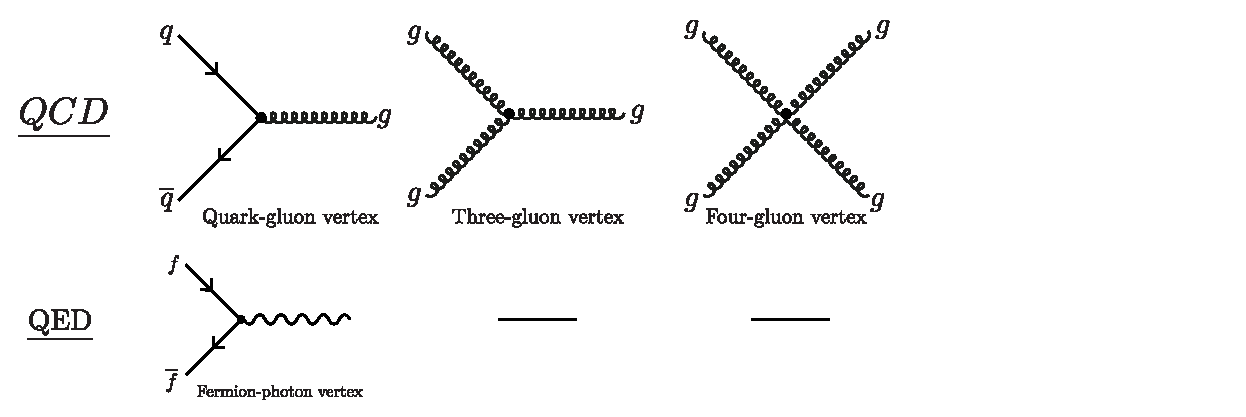
\includegraphics[width=\textwidth]{./images/qcdFeynmanDiagrams.eps}
%   \caption{Feynman diagrams of the strong interactions with corresponding
%   electromagnetic diagrams. We see that the gluons carry colour charge and
%   thus couple to other gluons, which is not the case for the photons.}
%   \label{fig:qcdFeynmanDiagrams}
% \end{figure}
\begin{table}
  \centering
  \begin{minipage}[c]{0.4\textwidth}
    \begin{tabular}{ll}
      \toprule
      Flavour & Mass\\
      \midrule
      $u$ & \SI{2.50(17)}{\mega\eV} \\
      $d$ & \SI{4.88(20)}{\mega\eV} \\
      $s$ & \SI{93.44(68)}{\mega\eV} \\
      $c$ & \SI{1.280(13)}{\giga\eV} \\
      $b$ & \SI{4.198(12)}{\giga\eV} \\
      $t$ & \SI{173.0(40)}{\giga\eV} \\
      \bottomrule 
    \end{tabular}
  \end{minipage}\hfill
  \begin{minipage}[c]{0.59\textwidth}
    \caption{List of quarks and their masses. The masses of the up, down and
      strange quark are quoted in the four\-/flavour theory (\(N_f=2+1+1\) at
      the scale \(\mu=\SI{2}{\giga\eV}\) in the \(\overline{MS}\). The charm and
      bottom quark are also taken in the four\-/flavour theory and in the
      \(\overline{MS}\) scheme, but at the scales \(\mu=m_c\) and \(\mu=\m_b\)
      correspondingly. All quarks except for the top quark are taken from the
      \textit{Flavour Lattice Averaging Group} \cite{FLAG2019}. The mass of the
      top quark is not discussed in \cite{FLAG2019} and has been taken from
      \cite{PDG2018} from direct observations of top events.}
  \end{minipage}
  \label{table:quarkList}
\end{table}
The classical \textit{Lagrange density} of \textsc{qcd} is given by
\cite{Yndurain2006,Pascual1984}:

\begin{tcolorbox}[ams equation,myformula]
  \label{eq:qcdLagrangian}
  \mathcal{L}_{QCD}(x) = -\frac{1}{4}G_{\mu\nu}^a(x)G^{\mu\nu a}(x) + \sum_A
  \left[ \frac{i}{2} \bar{q}^A(x) \gamma^\mu \overleftrightarrow{D}_\mu q^A(x) -
    m_A\bar{q}^A(x) a^A(x) \right],
\end{tcolorbox}
with $q^A(x)$ representing the quark fields and $G_{\mu\nu}^a$ being the
\textit{gluon field strength tensor} given by:
\begin{equation}
  \label{eq:gluonField}
  G_{\mu\nu}^a(x) \equiv \partial_\mu B_\nu^a(x) - \partial_\nu^a(x) + g f^{abc} B_\mu^b(x) B_\nu^c(x),
\end{equation}
with $f^{abc}$ as \textit{structure constants} of the gauge\-/group \(SU(3)\)
and \(\overleftrightarrow{D}_\mu\) as covariant derivative acting to the left
and to the right. Furthermore we have used $A, B, \dotsc = 0, \dotsc 5$ as
flavour indices, $a, b, \dotsc = 0, \dotsc, 8 $ as colour indices and $\mu, \nu,
\dotsc = 0, \dotsc 3$ as lorentz indices. Explicitly the Lagrangian writes:
\begin{equation}
  \begin{split}
    \mathcal{L}_0(x) &=- \frac{1}{4} \left[ \partial_\mu G_\nu^a(x) - \partial_v G_\mu^a(x) \right] \left[ \partial^\mu G_a^\nu(x) - \partial^\nu G^\mu_a(x) \right] \\
    &\quad+ \frac{i}{2}\anti{q}_\alpha^A(x) \gamma^\mu \partial_\mu q_\alpha^A(x) - \frac{i}{2} \left[ \partial_\mu \anti{q}_\alpha^A(x) \right] \gamma^\mu q_\alpha^A(x) - m_A \anti{q}_\alpha^A(x) q_\alpha^A(x) \\
    &\quad+ \frac{g_s}{2} \anti{q}_\alpha^A(x) \lambda^a_{\alpha \beta}\gamma_\mu q_\beta^A(x) G^\mu_a(x) \\
    &\quad- \frac{g_s}{2}f_{abc}\left[ \partial_\mu G_\nu^a(x) - \partial_\nu G_\mu^a(x)\right] G_b^\mu(x) G_c^\nu(x) \\
    &\quad- \frac{g_s^2}{4} f_{abc}f_{ade} G_\mu^b(x) G_\nu^c(x) G_d^\mu(x)
    G_e^\nu(x)
  \end{split}
\end{equation}
The first term is the kinetic term for the massless gluons. The next three terms
are the kinetic terms for the quark field with different masses for each
flavour. The rest of the terms are the interaction terms. The fifth term
represents the interaction between quarks and gluons and the last two terms the
self\-/interactions of gluon fields.

The corresponding Feynman rules have been displayed in
\cref{fig:qcdFeynmanRules}.
\begin{figure}
  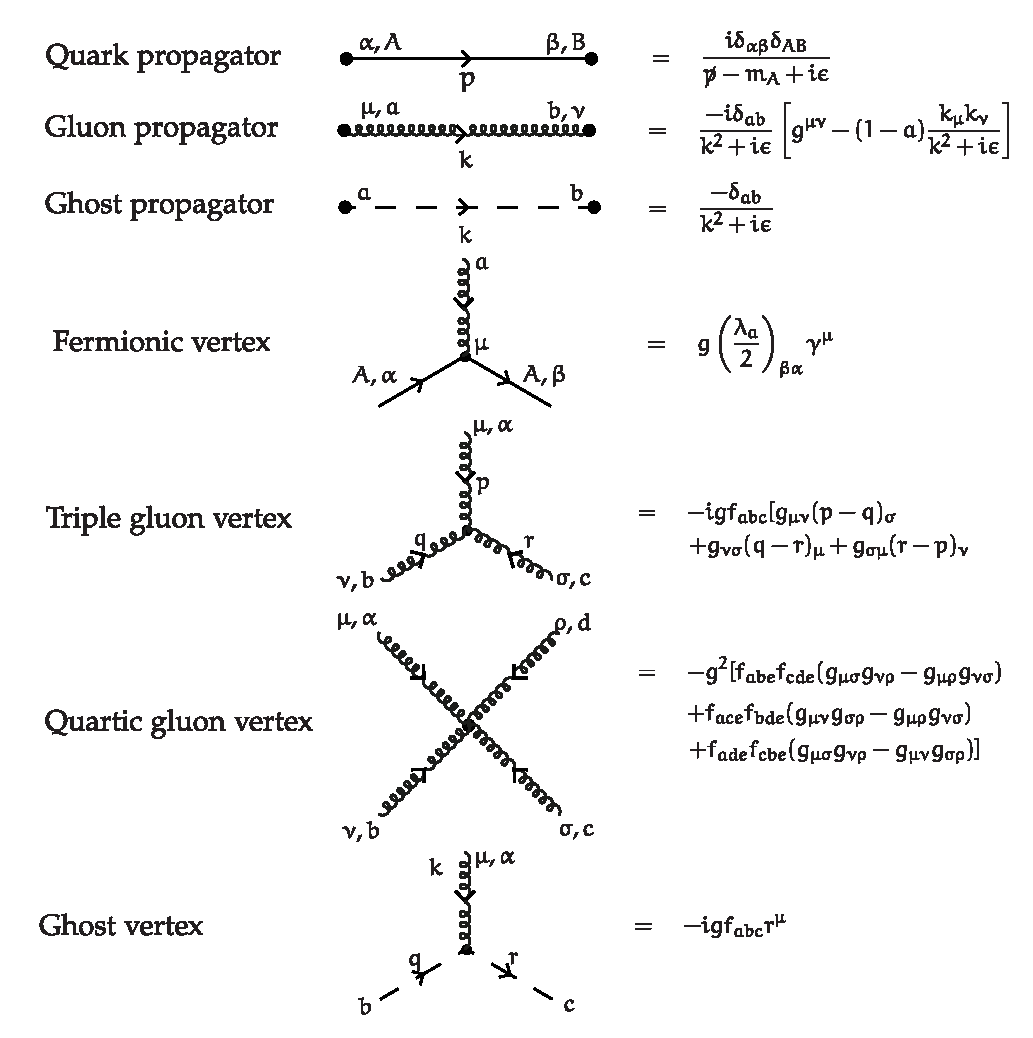
\includegraphics[width=\textwidth]{./images/qcdFeynmanRules.eps}
  \caption{QCD Feynman rules.}
  \label{fig:qcdFeynmanRules}
\end{figure}
The rules are based on \textsc{pt}, but can be enhanced with the \textsc{qcd}
condensates, as we will see in the discussion of the \textsc{ope} in
\cref{sec:ope}

Having derived the Lagrangian leaves us with its quantisation. The
dirac\-/spinors can be quantised as in \textsc{qed} without any problems. The
$\Psi(x)$ quantum field can be written as:
\begin{equation}
  \Psi(x) = \int \frac{\dif^3 p}{(2\pi)^3 2E(\vec p)} \sum_\lambda \left[ u(\vec p, \lambda) a(\vec p, \lambda) e^{-ipx} + v(\vec p, \lambda) b^\dagger (\vec p, \lambda) e^{ipx} \right],
\end{equation}
where the integration ranges over the positive sheet of the mass hyperboloid
$\Omega_+(m) = \{p \vert p^2 = m^2, p^0 > 0 \}$. The four spinors $u(\vec p,
\lambda)$ and $v(\vec p, \lambda)$ are solutions to the dirac equations in
momentum space
\begin{equation}
  \begin{split}
    [\slashed p - m]u(\vec p, \lambda) &= 0 \\
    [\slashed p + m]v(\vec p, \lambda) &= 0,
  \end{split}
\end{equation}
with $\lambda$ representing the helicity state of the spinors.

The quantisation of the gauge fields is more cumbersome. One is forced to
introduce supplementary non\-/physical fields, the so\-/called Faddeev\-/Popov
ghosts $c^a(x)$ \cite{Faddeev1967}, to cancel unphysical helicity degrees of
freedom of the gluon fields.

The free propagators for the quark, the gluon and the ghost fields are then
given by
\begin{equation}
  \begin{split}
    i S^{(0)AB}_{\alpha\beta}(x-y) &\equiv \wick{ \c q_\alpha^A(x) \anti{\c
        q}_\beta^B(y)} \equiv \langle 0 \vert T \{ q_\alpha^A(x)
    \anti{q}_\beta^B \} \vert 0 \rangle
    = \delta_{AB} \delta_{\alpha\beta} i S^{(0)}(x-y) \\
    &= i \delta_{AB}\delta_{\alpha\beta}\int \fdif{p} \frac{\slashed p + m}{(p^2 - m^2 + i\epsilon)}\\
    i D^{(0)\mu\nu}_{ab}(x-y) &\equiv \wick{ \c B_a^\mu(x) \c B_b^\nu(y)} \equiv
    \langle 0 \vert T \{ B_a^\mu(x) B_b^\nu(y) \} \vert 0 \rangle
    \equiv \delta_{ab}i \int \frac{\dif^4 k}{(2\pi)^4} D^{(0)\mu\nu}(k) e^{-ik(x-y)} \\
    &= i \delta_{ab} \int \frac{\dif^4 k}{(2\pi)^4} \frac{1}{k^2+i\epsilon} \left[ -g_{\mu\nu} + (1-a) \frac{k_\mu k_\nu}{k^2+i\epsilon} \right] e^{-ik(x-y)} \\
    i \widetilde{D}_{ab}^{(0)}(x-y) & \equiv \wick{\c \phi_a(x) \anti{\c
        \phi}_b(y)} \equiv \langle 0 \vert T\{ \phi_a(x) \anti{\phi}_b(y) \}
    \vert 0 \rangle
    = \frac{i}{(2\pi)^4}\delta_{ab} \int \dif^4 q \frac{-1}{q^2 + i\epsilon} e^{-q(x-y)} \\
    &\equiv \frac{i}{(2\pi)^4} \delta_{ab} \int \dif^4 q \widetilde{D}^{(0)}(q)
    e^{-iq(x-y)},
  \end{split}
\end{equation}

The previously introduced Feynman rules and propagators all make use of the
perturbative vacuum \(\vert 0 \rangle\) and are thus counted as tools of
\textsc{pt}. Consequently they need a small coupling to approximate excitations
of full \textsc{qcd} vacuum. We will see in the following section, that the
strong coupling runs with energy and unfortunately is large for small energy
scales.

\subsection{Renormalisation Group}
Computing observables with the \textsc{qcd} Lagrangian (\cref{eq:qcdLagrangian})
lead to divergencies, which have to be \textit{renormalised}. To render these
divergent quantities finite we have to introducing a suitable parameter such
that the ``original divergent theory'' corresponds to a certain value of that
parameter. These procedure is referred to as \textit{regularisation} and there
are various approaches:
\begin{itemize}
\item \label{itm:lambdaRegularisation}\textbf{Cut\-/off regularisation:} In
  cut\-/off regularisation we limit the divergent momentum integrals by a
  cut\-/off $\abs{\vec p} < \Lambda$. Here $\Lambda$ has the dimension of mass.
  The cut\-/off regularisation breaks translational invariance, which can be
  guarded by making use of other regularisation methods.
\item \textbf{\define{Pauli-Villars}{P-V} regularisation:} \cite{Pauli1949} In
  \textsc{P-V} regularisation the propagator is forced to decrease faster than
  the divergence to appear. It replaces the nominator by
  \begin{equation}
    (\vec p^2 + m^2)^{-1} \to (\vec p^2 + m^2)^{-1} - (\vec p^2 + M^2)^{-1},
  \end{equation}
  where $M$ has the dimension acts similar as the previously presented
  cut\-/off, but conserves translational invariance.
\item \textbf{Dimensional regularisation:}
  \cite{Bollini1972,tHooft1972,tHooft1973} Dimensional regularisation has been
  introduced in the beginning of the seventies to regularise non\-/abelian gauge
  theories (like \textsc{qcd}), where $\Lambda$\-/ and
  \textsc{P-V}\-/regularisation failed. In dimensional regularisation we expand
  the four space\-/time dimensions to arbitrary $D$-dimensions. To compensate
  for the additional dimensions we introduce an additional scale $\mu^{D-4}$. A
  typical Feynman\-/integral then has the following appearance:
  \begin{equation}
    \label{eq:dimRegFeynmanIntegral}
    \int \fdif{p} \frac{1}{\vec p^2 + m^2} \to \mu^{2\epsilon} \int \frac{\dif^D p}{(2\pi)^D}\frac{1}{\vec p^2+m^2},
  \end{equation}
  Dimensional regularisation preserves all symmetries, it allows an easy
  identification of divergences and naturally leads to the \define{ms}{minimal
    subtraction scheme} \cite{tHooft1973,Weinberg1973a}.
\end{itemize}
In all of the three regularisation schemes we introduced an arbitrary parameter
to regularise the divergence. This parameter causes scale dependence of the
strong coupling and the quark masses. As we are mainly concerned with the
non\-/abelian gauge theory \textsc{qcd} we will focus on dimensional
regularisation, which introduced the parameter $\mu$. Measurable observables
(\textit{Physical quantities}) cannot depend on the renormalisation scale $\mu$.
Therefore the derivative by $\mu$ of a general physical quantity has to yield
zero. A physical quantity $R(q, a_s, m)$, that depends on the external momentum
q, the renormalised coupling $a_s\equiv\alpha_s/\pi$ and the renormalised quark
mass $m$ can then be expressed as
\begin{equation}
  \label{eq:RGE}
  \mu \od{}{\mu}R(q, a_s, m) = \left[ \mu \pd{}{\mu} + \mu \od{a_s}{\mu} \pd{}{m} + \mu \od{m}{\mu} \pd{}{m} \right] R(q, a_s, m) = 0.
\end{equation}
\Cref{eq:RGE} is referred to as a \define{rge}{renormalisation group equation}
and is the basis for defining the two \textit{renormalisation group functions}:
\begin{align}
  \beta(a_s) &\equiv -\mu \od{a_s}{\mu} = \beta_1 a_s^2 + \beta_2 a_s^3 + \dots & \beta-\text{function}
                                                                                  \label{eq:betaFunction} \\
  \gamma(a_s) &\equiv - \frac{\mu}{m} \od{m}{\mu} = \gamma_1 a_s + \gamma_2 a_s^2 + \dots & \text{anomalous mass dimension}.
                                                                                            \label{eq:anomalousMassDimension}
\end{align}
The \(\beta\)\-/function dictates the running of the strong coupling, whereas
the anomalous mass dimension describes the running of the quark masses. We have
a special interest in the running of the strong coupling, but will also shortly
sum up the running of the quark masses.

\subsubsection{Running gauge coupling}
Regarding the $\beta$-function we notice, that $a_s(\mu)$ is not a constant, but
that it \textit{runs} by varying its scale $\mu$. To better understand the
running of the strong coupling we integrate the \(\beta\)\-/function
\begin{equation}
  \int_{a_s(\mu_1)}^{a_s(\mu_2)}\frac{\dif a_s}{\beta(a_s)} = - \int_{\mu_1}^{\mu_2} \frac{\dif \mu}{\mu} = \log \frac{\mu_1}{\mu_2}.
\end{equation}
To analytically evaluate the above integral we can approximate the
$\beta$-function to first order, with the known coefficient
\begin{equation}
  \label{eq:firstBetaCoefficient}
  \beta_1 = \frac{1}{6}(11 N_c - 2 N_f),
\end{equation}
yielding
\begin{equation}
  \label{eq:strongCouplingFirstOrder}
  a_s(\mu_2) = \frac{a_s(\mu_1)}{\left( 1 - a_s(\mu_1) \beta_1 \log\frac{\mu_1}{\mu_2} \right)}.
\end{equation}

\begin{figure}
  \centering \includegraphics[width=\textwidth]{./images/runningOfAs.eps}
  \caption{Running of the strong coupling \(\alpha_s(Q^2)\) at first order. The
    blue line represents the uncorrected coupling constant, with an
    \(\Lambda^{nf=5}\) chosen to match an experimental value of the coupling at
    \(Q^2=M_Z^2\). The quark\-/thresholds are shown by the black line and the
    corrected running is given by the red line. We additionally marked the
    breakdown of \text{pt} with a grey background for \(Q^2<1\). The image is
    taken from an recent review of the strong coupling \cite{Deur2016}.}
  \label{fig:runningOfAs}
\end{figure}

\Cref{eq:strongCouplingFirstOrder} has some important implications for the
strong coupling:
\begin{itemize}
\item The coupling at a scale \(\mu_2\) depends on \(a_s(\mu_1)\). Thus we have
  to take care of the scale \(\mu\), while comparing different values of
  \(\alpha_s\). In the literature (e.g. \cite{pdg2016}) \(\alpha_s\) is commonly
  compared at the \(Z\)\-/boson scale of around \SI{91}{\giga\eV}. As we are
  extracting the strong coupling at the mass of the tau lepton, around
  \SI{1.776}{\giga\eV} we need to run the strong coupling up to the desired
  scale. While running the coupling, we have to take care of the
  quark\-/thresholds. Each quark gets active at a certain energy scale, which
  leads to a running of \(\alpha_s\) as shown in \cref{fig:runningOfAs}.
  Typically one runs the coupling with the aid of software packages like
  \textit{RunDec} \cite{Chetyrkin2000,Herren2017}, which has also been ported to
  support \(C\) (\textit{CRunDec}, \cite{Schmidt2012}) and Python
  \cite{Straub2016}.
\item As we have three colours (\(N_c=3\) and six flavours (\(N_f=6\) the first
  \(\beta_1\) coefficient \ref{eq:betaFunction} is positive. Thus for
  \(\mu_2<\mu_1\) \(a_s(\mu_2)\) increases logarithmically and at a scale of
  \(\mu_2=\SI{1}{\giga\eV}\) reaches a value of
  \begin{equation}
    \alpha_s(\SI{1}{\giga\eV}) \approx 0.5,
  \end{equation}
  which questions the applicability of \textsc{pt} for energies lower than
  \SI{1}{\giga\eV} (as seen from the grey zone in \cref{fig:runningOfAs}).
\item A large coupling for small scales implies confinement. We are not able to
  separate quarks in a meson or baryon. No quark has been detected as single
  particle yet. This is qualitatively explained with the gluon field carrying
  colour charge. These gluons form so-called \textit{flux-tubes} between quarks,
  which cause a constant strong force between particles regardless of their
  separation. Consequently the energy needed to separate quarks is proportional
  to the distance between them and at some point there is enough energy to
  favour the creation of a new quark pair. Thus before separating two quarks we
  create a quark\-/antiquark pair. As a result we will probably never be able to
  observe an isolated quark. This phenomenon is referred to as colour
  confinement or simply confinement.
\item With the first \(beta_1\) coefficient being positive we notice that for
  increasing scales (\(\mu_2>\mu_1\)) the coupling decreases logarithmically.
  This leads to asymptotic freedom, which states, that for high energies (small
  distances), the strong coupling becomes diminishing small and quarks and
  gluons do not interact. Thus in isolated baryons and mesons the quarks are
  separated by small distances, move freely and do not interact. \end{itemize}

From the \textsc{rge} we have seen, that not only the coupling but also the
masses carry an energy dependencies.

\subsubsection{Running quark mass}
The mass dependence on energy is governed by the \textit{anomalous mass
  dimension} $\gamma(a_s)$. Its properties of the running quark mass can be
derived similar to the gauge coupling. Starting from integrating the
\textit{anomalous mass dimension} \cref{eq:anomalousMassDimension}
\begin{equation}
  \log \frac{m(\mu_2)}{m(\mu_1)} = \int_{a_s(\mu_1)}^{a_s(\mu_2)} \dif a_s \frac{\gamma(a_s)}{\beta(a_s)}
\end{equation}
we can approximate the \textit{anomalous mass dimension} to first order and
solve the integral analytically \cite{Schwab2002}
\begin{equation}
  m(\mu_2) = m(\mu_1)\left( \frac{a(\mu_2)}{a(\mu_1)} \right)^{\frac{\gamma_1}{\beta_1}} \left( 1 + \mathcal{O}(\beta_2, \gamma_2) \right).
\end{equation}
As $\beta_1$ and $\gamma_1$ (see \ref{app:gammaCoefficients}) are positive the
quark mass decreases with increasing $\mu$. The general relation between
different scales is given by
\begin{equation}
  m(\mu_2) = m(\mu_1) \exp \left( \int_{a_s(\mu_1)}^{a_s(\mu_2)} \dif a_s \frac{\gamma(a_s)}{\beta(a_s)}  \right)
\end{equation}
and can be solved numerically to run the quark mass to the needed scale $\mu_2$.
Both, the \(\beta\)\-/function and the anomalous mass dimension are currently
known up to the 5\textsuperscript{th} order and listed in the appendix
\ref{sec:betaCoefficients}.

\textsc{qcd} in general has a precision problem caused by uncertainties and
largeness of the strong coupling constant $\alpha_s$. The fine-structure
constant (the coupling \textsc{qed}) is known to eleven digits, whereas the
strong coupling is only known to about four. Furthermore for low energies the
strong coupling constant is much larger than the fine-structure constant. E.g.
at the $Z$-mass, the standard mass to compare the strong coupling, we have an
$\alpha_s$ of $0.11$, whereas the fine structure constant would be around
$0.007$. Consequently to use \textsc{pt} we have to calculate our results to
much higher orders, including tens of thousands of Feynman diagrams, in
\textsc{qcd} to achieve a precision equal to \textsc{qed}. For even lower
energies, around \SI{1}{\giga\eV}, the strong coupling reaches a critical value
of around \(0.5\) leading to a break down of \textsc{pt}.

In this work we try to achieve a higher precision in the value of $\alpha_s$.
The framework we use to measure the strong coupling constant are the
\textsc{qcdsr}. A central object needed to describe hadronic states with the
help of \textsc{qcd} is the \textit{two-point function} for which we will devote
the following section.

\section{Two-Point function}
\label{sec:twoPointFunction}
A lot of particle physics is dedicated to calculating the \textit{S\-/matrix},
which contains all the information about how initial states evolve in time. One
important tool for obtaining the S\-/matrix is the \textit{LSZ
  (Lehmann\-/Symanzik\-/Zimmermann)-reduction formula}
\cite{Lehmann1954a,Schwartz2013}
\begin{equation}
  \begin{split}
    \langle f\vert S \vert i\rangle = \left[ i\int_0^\infty \fdif{x_1}
      e^{-ip_1x_1} (\Box^2 + m^2)\right] \cdots
    \left[ i\int_0^\infty \fdif{x_n} e^{ip_nx_n} (\Box^2 + m^2)\right] \\
    \times \langle\Omega\vert T\{\phi(x_1)\cdots\phi(x_n)\} \vert\Omega\rangle,
  \end{split}
\end{equation}
with the $-i$ in the exponent applying for initial states and the $+i$ for final
states. The LSZ\-/reduction formula relates the S\-/matrix to the
\textit{correlator} (also referred to as \textit{n\-/point function})
\begin{equation}
  \langle\Omega\vert T\{\phi(x_1)\phi(x_2)\cdots\phi(x_n)\} \vert\Omega\rangle,
\end{equation}
where $T\{\cdots\}$ is the time\-/ordered product and $\vert\Omega\rangle$ is
the ground state/ vacuum of the interacting theory. Note that the fields are in
general given in the Heisenberg picture, which implies translational invariance.
\begin{equation}
  \begin{split}
    \langle\Omega\vert \phi(x)\phi(y) \vert\Omega\rangle &= \langle\Omega\vert \phi(x) e^{i\hat P y}e^{-i\hat P y}\phi(y)e^{i\hat P y}e^{-i\hat P y} \vert\Omega\rangle \\
    &= \langle\Omega\vert \phi(x-y)\phi(0) \vert\Omega\rangle,
  \end{split}
\end{equation}
where we made use of the translation operator $\hat T(x) = e^{-i \hat P x}$.

In this work we are solely concerned about the \textit{two\-/point function},
especially in the vacuum expectation value of the Fourier transform of two
time\-/ordered \textsc{qcd} quark Noether currents
\begin{tcolorbox}[ams equation,myformula]
  \label{eq:qcdCorrelator}
  \Pi_{\mu\nu}(q^2) \equiv \int \fdif{q} e^{iqx} \langle\Omega\vert
  J_\mu(x)J_\nu(0) \vert\Omega\rangle,
\end{tcolorbox}
where the Noether current is given by
\begin{equation}
  \label{eq:qcdCurrent}
  J_\mu(x) = \anti{q}(x) \Gamma q(x).
\end{equation}
Here, $\Gamma$ can be any of the following dirac matrices $\Gamma \in \{ 1,
i\gamma_5, \gamma_\mu, \gamma_\mu\gamma_5\}$, specifying the quantum number of
the current (S: \textit{scalar}, P: \textit{pseudo-Scalar}, V:
\textit{vectorial}, A: \textit{axial-vectorial}, respectively). By choosing the
right quantum numbers we can theoretically represent the processes we want to
study, which will be important when we want to theoretically describe the
hadrons produced in $\tau$\-/decays.

\begin{wrapfigure}{r}{4cm}
  \centering
  \begin{tkizpicture}
    \feynmandiagram [small, vertical=a to b] { i1 [particle=\(\tau\)] -- [anti
      fermion] a -- [anti fermion] i2 [particle=\(\nu_\tau\)], a -- [scalar] b,
      b -- [fermion, half left, edge label=\(\anti{q}\)] c -- [fermion, half
      left, edge label=\(q\)] b, c -- [scalar] d, f1 [particle=\(\tau\)]--
      [fermion] d -- [fermion] f2 [particle=\(\nu_\tau\)], };
  \end{tkizpicture}
  \caption{\(\tau\anti{\tau}\)\-/annihilation with a quark\-/antiquark pair.}
  \label{fig:tauAntiTauAnnihilation}
\end{wrapfigure}
From a Feynman diagram point of view we can illustrate the two\-/point function
as quark\-/antiquark pair, which is produced by an external source, e.g. the
virtual \(W\)\-/boson of \(\tau\anti{\tau}\)\-/annihilation as seen in
\cref{fig:tauAntiTauAnnihilation}. Here the quarks are propagating at
\textit{short\-/distances}, which implies that we can make use of \textsc{pt},
thus avoiding \textit{long\-/distance} (\textsc{npt}\-/) effects, that would
appear if the initial and final states where given by hadrons
\cite{Colangelo2000}. It is interesting to note, that the same process with the
help of the \textit{optical theorem} can be used to derive the total decay width
of hadronic tau decays.

\subsection{Short\-/Distances vs. Long\-/Distances}
If we want to calculate the two\-/point function in \textsc{qcd} we have to
differentiate short\-/ and long\-/distances or large or small momenta. In
general when we talk about small distances we refer to large momenta. Large
momenta implies a small strong coupling constant. Consequently we can use
\textsc{pt} for short\-/distances without problems. On the contrary long
distances involve small momenta, which implies a large coupling constant. Thus
for long distances the \textsc{np} effects become important and have to be dealt
with. To apply \textsc{pt} to the case of the \(\tau\anti{\tau}\) annihilation
we need the quark\-/antiquark pair of \cref{fig:electronElectronScattering} to
be highly virtual \footnote{Which is the same of saying, that the
  quark\-/antiquark pair needs a high external momentum \(q\).}. To roughly
separate long\-/distances from short\-/distances using a length scale we can say
that the length scale should be smaller than the radius of a hadron.

\subsection{Relating Two\-/Point Function and Hadrons}
The two\-/point function can be interpreted physically as the amplitude of
propagating single- or multi\-/particle states and their excitations. The
possible states, in our case, the hadrons we describe through the correlator are
fixed by the quantum numbers of the current we define for the vacuum expectation
value. For example the neutral $\rho$\-/meson is a spin\-/1 vector meson with a
quark content of \((u\anti{u} - d\anti{d})/\sqrt{2}\). Consequently by choosing
a current
\begin{equation}
  J_\mu(x) = \frac{1}{2} ( \anti{u}(x)\gamma_\mu u(x) - \anti{d}(x)\gamma_\mu d(x) )
\end{equation}
the two\-/point function contains the same quantum numbers as the
\(\rho\)\-/meson and is said to materialise to it. A list of some ground\-/state
mesons for combinations of the light quarks \(u, d\) and \(s\) is given in
\cref{table:groundStateMesons}.
\begin{table}
  \centering
  \begin{tabular*}{\textwidth}{lccc @{\extracolsep{\fill}}c}
    \toprule
    Symbol & Quark content & Isospin & \(J\) & Current \\
    \midrule
    \(\pi^0\)  & \(\frac{u\anti{u} - d\anti{d}}{2}\) & \(1\) & \(0\)
    & :\(\anti{u}\gamma_\mu\gamma_5 u + \anti{d}\gamma_\mu\gamma_5 d\): \\
    \(\eta\)   & \(\frac{u\anti{u} + d\anti{d} - 2s\anti{s}}{\sqrt{6}}\) & \(0\)
    & \(0\) & :\(\anti{u}\gamma_\mu\gamma_5 u + \anti{d}\gamma_\mu\gamma_5d
    - 2\anti{s}\gamma_\mu\gamma_5 s\): \\
    \(\eta\prime\) & \(\frac{u\anti{u} + d\anti{d} + s\anti{s}}{\sqrt{3}}\)
    & \(0\) & \(0\) & :\(\anti{u}\gamma_\mu\gamma_5 u +
    \anti{d}\gamma_\mu\gamma_5 d + \anti{s}\gamma_\mu\gamma_5 s\): \\
    \(\rho^0\) & \(\frac{u\anti{u} - d\anti{d}}{\sqrt{2}}\) & \(1\) & \(1\)
    & :\(\anti{u}\gamma_\mu u - \anti{d}\gamma_\mu d\): \\
    \(\omega\) & \(\frac{u\anti{u}+d\anti{d}}{\sqrt{2}}\) & \(0\) & \(1\)
    & :\(\anti{u}\gamma_\mu u + \anti{d}\gamma_\mu d\): \\
    \(\phi\) & \(s \anti{s}\) & \(0\) & \(1\)
    & :\(\anti{s}\gamma_\mu\gamma_5 s\): \\                                        
    \bottomrule
  \end{tabular*}
  \caption{Ground\-/state vector and pseudoscalar mesons for the light\-/quarks
    \(u, d\) and \(s\) with their corresponding currents in the two\-/point
    function. Note that we use \(\gamma_\mu\) for vector and
    \(\gamma_\mu\gamma_5\) for the pseudoscalar mesons.}
  \label{table:groundStateMesons}
\end{table}

The correlator is materialising into a spectrum of hadrons. Thus if we insert a
complete set of states of hadrons we can make use of the unitary relation
\begin{equation}
  \langle\Omega\vert J_\mu(x)\J_\nu(0) \vert\Omega\rangle = \sum_X \langle\Omega\vert J_\mu(x) \vert X\rangle \langle X\vert J_\nu(0) \vert\Omega\rangle.
\end{equation}
to represent the two\-/point correlator via a spectral function \(\rho(t)\)
\begin{tcolorbox}[ams equation,myformula]
  \label{eq:KallenLehmannSpectralDecomposition}
  \Pi(q^2) = \int_0^\infty \dif s \frac{\rho(s)}{s-p^2-i\epsilon}.
\end{tcolorbox}
The above relation is referred to as \textit{Källén-Lehmann spectral
  representation} \cite{Kallen1952,Lehmann1954} or \textit{dispersion relation}.
It relates the two\-/point function to the spectral function $\rho$, which can
be represented as sum over all possible hadronic states
\begin{equation}
  \rho(s) = (2\pi)^3 \SumInt_X \abs{\langle\Omega\vert J_{\mu}(0) \vert X\rangle}^2 \delta^4(s-p_X).
\end{equation}
Note that the analytic properties of the two\-/point are in one\-/to\-/one
correspondence with the newly introduced spectral function and thus determined
by the possible hadrons states, which only form on the positive real axis. A
full derivation of the \textit{Källén\-/Lehmann spectral representation} can be
found in the appendix \cref{ch:kallenLehmannSpectralRepresentation}. We will
derive the same representation to a later point by solely using the analytic
properties of the correlator (see. \cref{sec:sumRules}). The spectral function
is interesting to us for two reasons. First it is experimentally measurable and
second it carries a problematic ``branch cut'', which we want to discuss now.

\subsection{Analytic Structure of the Two\-/Point Function}
The general two\-/point function $\rho(s)$ has some interesting, but problematic
analytic properties. It has poles for single\-/particle states and a continuous
branch cut for multi\-/particle states. The single and multi\-/particle states,
for a general correlator, can be mathematically separated by
\begin{equation}
  \rho(s) = Z \delta(s-m^2) + \theta(s-s_0)\sigma(s)
  + \sigma(s),
\end{equation}
where the second term is the contribution from multi\-/particle states.
\(\sigma(s)\) is zero till we reach the threshold, where we have sufficient
energy to form multi\-/particle states. The analytic structure is depicted by
\cref{fig:analyticStructureCorrelator} and we can see that the spectral function
has \(\delta\)\-/spikes for single\-/particle states and a continuous
contribution for \(s\geq 4m\) resulting from multi\-/particle states. These lead
to poles and a continuous branch cut of the two\-/point function.
\begin{figure}
  \centering
  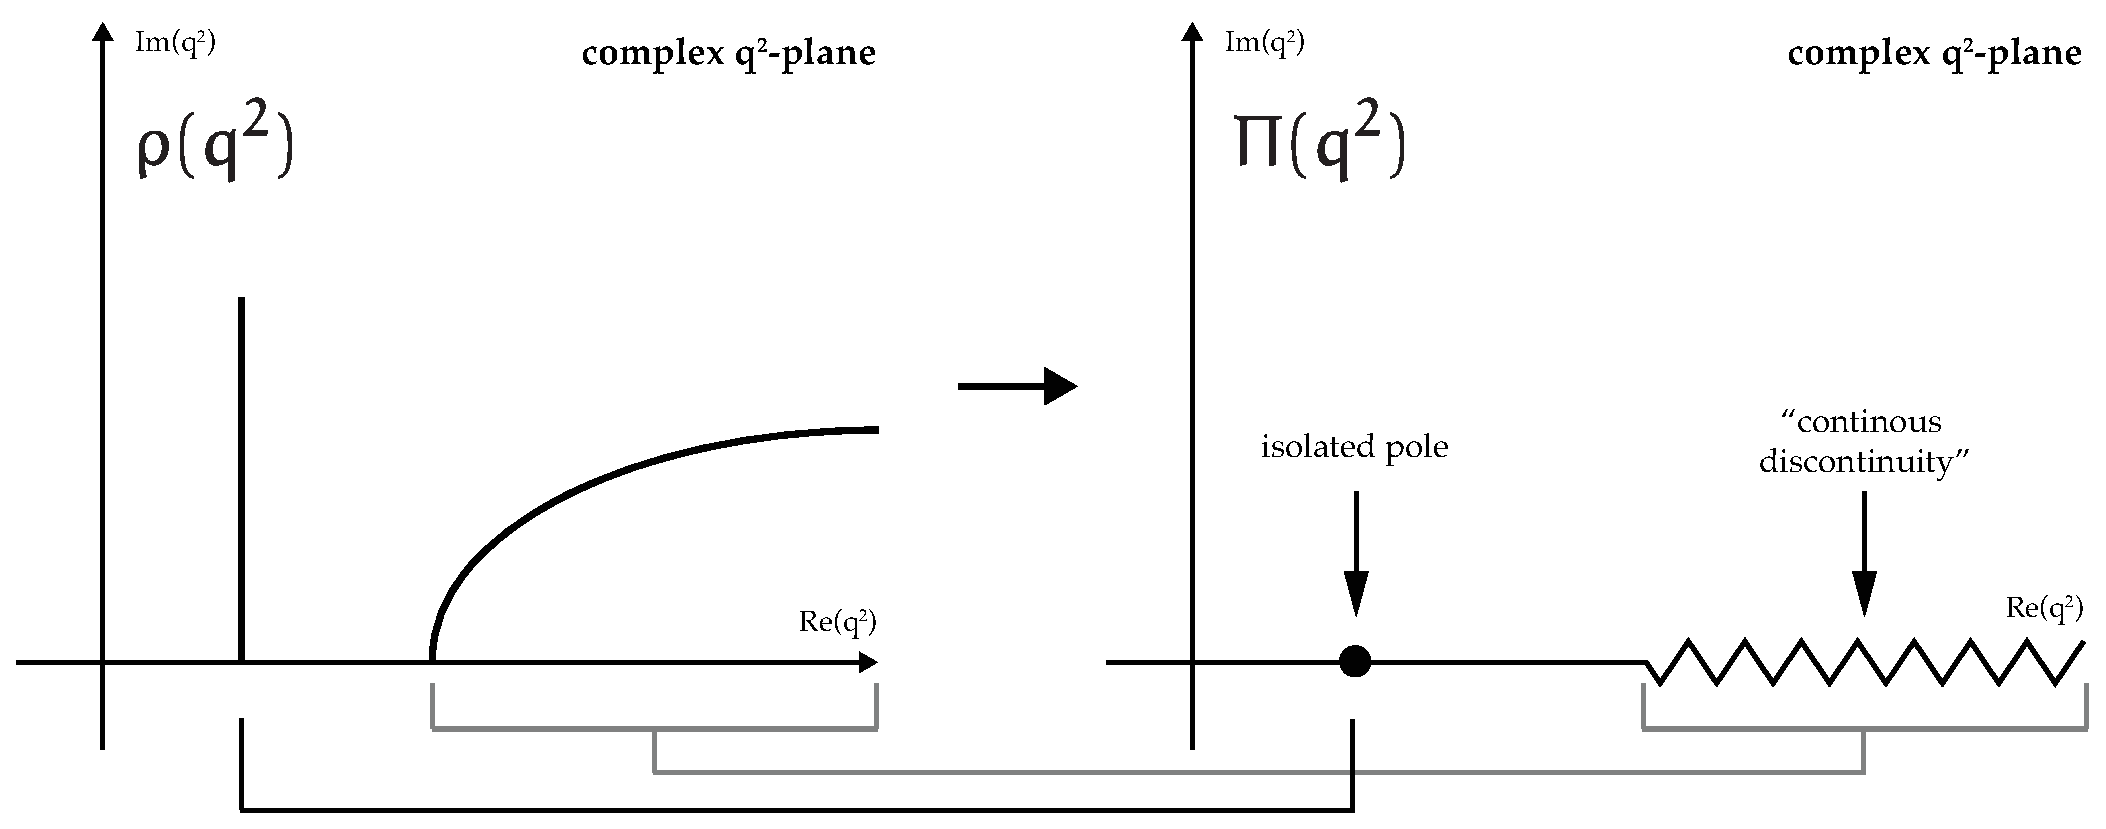
\includegraphics[width=\textwidth]{./images/analyticStructureCorrelator.eps}
  \caption{Analytic structure in the complex $q^2$-plane of the Fourier
    transform of the two-point function. The hadronic final states are
    responsible for poles appearing on the real-axis. The one-particle states
    contribute as isolated pole and the multi-particle states contribute as
    bound-states poles or a continues ``discontinuity cut''
    \cite{Peskin1995,Zwicky2016}.}
  \label{fig:analyticStructureCorrelator}
\end{figure}

\subsection{Lorentz Decomposition}
Apart the spectral decomposition we can Lorentz decompose the correlator to a
scalar function $\Pi(q^2)$. Due to Lorentz invariance, there exist only two
possible terms that can guard the structure of the second order tensor: $q_\mu
q_\nu$ and $q^2 g_{\mu\nu}$. The sum of both multiplied with two arbitrary
functions $A(q^2)$ and $B(q^2)$ yields
\begin{equation}
  \Pi_{\mu\nu}(q^2) = q_\mu q_\nu A(q^2) + q^2 g_{\mu\nu} B(q^2).
\end{equation}
By making use of the \textit{Ward\-/identity}
\begin{equation}
  \label{eq:wardIdentity}
  q^\mu \Pi_{\mu\nu} = 0
\end{equation} 
% \begin{equation}
%   \label{eq:wardIdentity}
%   \begin{split}
%     q^\mu \Pi_{\mu\nu} &= \int \dif x q^\mu e^{iqx} \langle 0 \vert  J_\mu(x) J_\nu(0) \vert 0 \rangle \\
%     &= -i \int \dif x i q^\mu e^{i q^\nu x_\nu} \langle 0 \vert J_\mu(x) J_\nu(0) \vert 0 \rangle \\
%     &= i \int \dif x e^{iqx} \langle 0 \vert \partial_\mu[J_\mu(x)] J_\nu(0)
%     \vert 0 \rangle \\
%     &= 0, \quad \text{with} \quad \partial_\mu J_\mu(x) = 0,
%   \end{split}
% \end{equation}
% where we used $i q^\mu e^{i q^\nu x_\nu} = \partial_\mu e^{i q^\nu x_\nu}$ in
% the second and integration by parts in the third line.
The Ward identity is dependent on the conserved Noether\-/current $J_\mu$ and
thus only holds for same flavour quarks. With the Ward\-/identity we are able to
demonstrate, that the two arbitrary functions are related
\begin{equation}
  \begin{split}
    q^\mu q^\nu \Pi_{\mu\nu} &= q^4 A(q^2) + q^4 B(q^2) = 0 \\
    &\quad \implies A(q^2) = -B(q^2).
  \end{split}
\end{equation}
Thus redefining $A(q^2) \equiv \Pi(q^2)$ we expressed the correlator as a scalar
function
\begin{equation}
  \Pi_{\mu\nu}(q^2) = (q_\mu q_\nu - q^2 g_{\mu\nu})\Pi(q^2).
\end{equation}

\subsection{More Decompositions}
\textcolor{red}{compositions check!} The two-point function can be Lorentz
decomposed, but we can also decompose it into its transversal and longitudinal
components. Both, the longitudinal and transversal components are related and
have implications for a common used approximation: the \textbf{chiral limit},
where the quark masses are taken to zero (\(m_q \to 0\)).

Starting with the decomposition into \define{V}{vector},
\define{A}{axial\-/vector}, \define{S}{scalar} and \define{P}{pseudo-scalar}
components we can write \cite{Broadhurst1981,Jamin1992}
\begin{equation}
  \label{eq:correlatorVectorScalarDecomposition}
  \begin{split}
    \Pi^{\mu\nu}(q^2) &= (q^\mu q^\nu - q^2 g^{\mu\nu}) \Pi^{V,A}(q^2) + \frac{g^{\mu\nu}}{q^2} (m_i \mp m_j)\Pi^{S,P}(q^2) \\
    &+ g^{\mu\nu}\frac{(m_i \mp m_j)}{q^2} [ \langle\Omega\vert \anti{q}_i q_i
    \vert\Omega\rangle \mp \langle\Omega\vert \anti{q}_j q_j
    \vert\Omega\rangle],
  \end{split}
\end{equation}
which is composed of a vector $\Pi^{V,A}$ and scalar $\Pi^{S,P}$ part. The third
term is a correction arising due to the physical vacuum $|\Omega\rangle$. The
latter decomposition rewrites the correlator $\Pi^{\mu\nu}(q^2)$ into
transversal and longitudinal components:
\begin{equation}
  \label{eq:correlatorTransversalLongitudinalDecomposition}
  \Pi^{\mu\nu}(q^2) = (q^\mu q^\nu - g^{\mu\nu}q^2) \Pi^{(1)}(q^2) + q^\mu q^\nu \Pi^{(0)}(q^2).
\end{equation}
With the two decompositions \cref{eq:correlatorVectorScalarDecomposition} and
\cref{eq:correlatorTransversalLongitudinalDecomposition} we can now identify the
longitudinal components of the correlator as being purely scalar, by multiplying
\cref{eq:correlatorVectorScalarDecomposition} by two four-momenta and making use
of the Ward-idendity \cref{eq:wardIdentity} we can write
\begin{equation}
  q_\mu q_\nu \Pi^{\mu\nu}(q^2) = (m_i \mp m_j)^2 \Pi^{S,P}(q^2) + (m_i \mp m_j)[\langle \anti{q}_i q_i \rangle \mp \langle \anti{q}_j q_j \rangle],
\end{equation}
which then can be related to the longitudinal component of
\cref{eq:correlatorTransversalLongitudinalDecomposition} by comparison of the
two equations
\begin{equation}
  q_\mu q_\nu \Pi^{\mu\nu}(q^2) = q^4 \Pi^{(0)}(q^2) = s^2 \Pi^{(L)}(s) \quad \text{with} \quad s\equiv q^2.
\end{equation}
In a more eloquent way this can be expressed as
\begin{equation}
  \label{eq:longitudinalTwoPointFunction}
  s^2 \Pi^{(0)}(s) = (m_i \mp m_j)^2 \Pi^{(S,P)}(s) + (m_i \mp m_j)[ \langle \anti{q}_i q_i \rangle \mp \langle \anti{q}_j q_j \rangle],
\end{equation}
where we can see, that all mass terms are related to the longitudinal component
of the correlator.

We note, that the longitudinal component in
\cref{eq:longitudinalTwoPointFunction} and the scalar component in
\cref{eq:correlatorVectorScalarDecomposition} vanish in the chiral limit, which
will become handy in the next chapter.

By defining a combination of the transversal and longitudinal correlator
\begin{equation}
  \label{eq:correlatorCombination}
  \Pi^{(1+0)}(s) \equiv \Pi^{(1)}(s) + \Pi^{(0)}(s)
\end{equation}
we can additionally relate the transversal and vectorial components via
\begin{equation}
  \label{eq:longitudinalCorrelator}
  \begin{split}
    \Pi^{\mu\nu}(s) &= \underbrace{(q^\mu q^\nu - g^{\mu\nu}q^2)\Pi^{(1)}(s) +
      (q^\mu q^\nu - g^{\mu\nu} q^2)\Pi^{(1)}(s)}_{=(q^\mu q^\nu - g^{\mu\nu}
      q^2) \Pi^{(1+0)}(s)} + \frac{g^{\mu\nu}s^2}{q^2}\Pi^{(0)}(s),
  \end{split}
\end{equation}
such that
\begin{equation}
  \Pi^{(V,A)}(s) = \Pi^{(1)}(s) + \Pi^{(0)} = \Pi^{(1+0)},
\end{equation}
where the vector/ axial-vector component of the correlator is now related to the
newly defined transversal and longitudinal combination of the correlator. As the
tau decays, with the limiting factor of the tau mass, can only decay into light
quarks we will often neglect the quark masses and work in the so called chiral
limit. In the chiral limit the longitudinal component of the correlator, which
is proportional to the quark masses, vanishes.

Having dealt exclusively with the perturbative part of the theory, we have to
discuss \textsc{np} contributions. These arise due to non negligible
long\-/distance effects. Thus to complete the needed ingredients for \textit{Sum
  Rules} we need a final ingredient the \define{ope}{Operator Product
  Expansion}, which treats the non\-/perturbative contributions of our theory.


\section{Operator Product Expansion}
\label{sec:ope}
The \textsc{ope} was introduced by Wilson in 1969 \cite{Wilson1969} as an
alternative to the in this time commonly used current\-/algebra. The expansion
states that non\-/local operators can be rewritten into a sum of composite local
operators and their corresponding coefficients:
\begin{tcolorbox}[ams equation,myformula]
  \label{eq:ope}
  \lim_{x\to y} A(x) B(y) = \sum_n C_n(x-y)\mathcal{O}_n(x),
\end{tcolorbox}
where $C_n(x-y)$ are the so-called \textit{Wilson-coefficients} and \(A, B\) and
\(\mathcal{O}_n\) are operators.

The OPE lets us separate short distances from long distances. In pure
\textsc{pt} we can only amount for short distances, which are equal to high
energies, where the strong-coupling $\alpha_s$ is small. The \textsc{ope} on the
other hand accounts for long\-/distance effects with higher dimensional
operators.

The form of the composite operators are dictated by gauge- and Lorentz symmetry.
Thus we can only make use of operators of even dimension. The scalar operators
up to dimension six are given by \cite{Pascual1984}
\begin{equation}
  \begin{array}{ll}
    \text{Dimension 0:} & \mathbb{1} \\
    \text{Dimension 4:} & :m_i \anti{q} q: \\
                        & :G_a^{\mu\nu}(x) G_{\mu\nu}^a(x): \\
    \text{Dimension 6:} & :\anti{q} \Gamma q \anti{q} \Gamma q: \\
                        & :\anti{q} \Gamma \frac{\lambda^a}{2} q_\beta(x) \anti{q} \Gamma \frac{\lambda^a}{2} q: \\
                        & :m_i \anti{q} \frac{\lambda^a}{2} \sigma_{\mu\nu} q G^{\mu\nu}_a: \\
                        & :f_{abc} G_a^{\mu\nu} G_b^{\nu\delta} G_c^{\delta\mu}:,
  \end{array}
\end{equation}
where $\Gamma$ stands for one of possible dirac matrices (as seen
\cref{eq:qcdCurrent}). The operator of dimension zero is the identity and its
Wilson\-/coefficient is solely perturbative. The higher dimension operators
appear as normal ordered products of fields and vanish by being sandwiched into
the perturbative vacuum. On the contrary, in \textsc{np qcd} they appear as
\textit{condensates}. Condensates are the vacuum expectation values of
non\-/vanishing normal ordered fields by applying the full \textsc{qcd} vacuum,
which contribute to all strong processes. For example the condensates of
dimension four are the quark-condensate $\langle \anti{q} q \rangle$ and the
gluon-condensate $\langle GG \rangle$.

As we work with dimensionless functions (e.g. the correlator $\Pi$), the r.h.s.
of \cref{eq:ope} has to be dimensionless. As a result the Wilson-coefficients
have to cancel the dimension of the operator with their inverse mass dimension.
To account for the dimensions we can make the inverse momenta explicit
\begin{equation}
  \Pi_{V/A}^{OPE}(s) = \sum_{D=0,2,4\dots} \frac{c^{(D)} \langle \mathcal{O}^{(D)}(x) \rangle}{(-q^2)^{D/2}},
\end{equation}
where we used $C^{(D)}=c/(-s)^{D/2}$ with $D$ being the dimension. Thus the
\textsc{ope} should converge with increasing dimension for sufficiently large
momenta $s$.

\subsection{A practical example}
Let's show how the \textsc{ope} contributions are calculated \cite{Shifman1978,
  Pascual1984}. We will compute the perturbative and quark-condensate
Wilson-coefficients for the rho meson. To do so we have to evaluate Feynman
diagrams using standard \textsc{pt}.

The rho meson is a vector meson of isospin one composed of \(u\) and \(d\)
quarks. As a result (see. \cref{table:groundStateMesons}) we can match its
quantum numbers with the current
\begin{equation}
  J^\mu(x) = \frac{1}{2}\left(:[\anti{u} \gamma^\mu u](x) - [\anti{d} \gamma^\mu d](x):\right).
\end{equation}
\begin{figure}
  \centering
  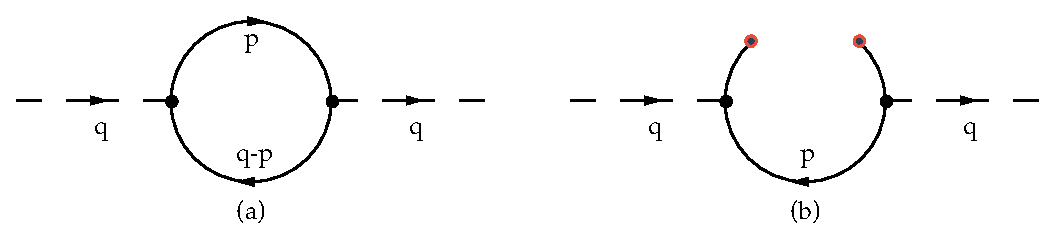
\includegraphics[width=\textwidth]{./images/condensateFeynmanDiagram.eps}
  \caption{Feynman diagrams of the perturbative (a) and the quark-condensate (b)
    contribution. The upper part of the right diagram is not wick-contracted and
    responsible for the condensate.}
  \label{fig:OPEFeynmanDiagram}
\end{figure}
Pictorial the dimension zero contribution is given by the quark\-/antiquark loop
Feynman diagram \cref{fig:OPEFeynmanDiagram}. The higher dimension contributions
are given by the same Feynman diagram, but with non contracted fields. These non
contracted fields contain the condensates. Thus not contracting the
quark\-/antiquark field (see. \cref{fig:OPEFeynmanDiagram} b) will give us
access to the Wilson coefficient of the dimension four quark\-/condensate
\(\langle \anti{q}q \rangle\).

The perturbative part (the Wilson coefficient of dimension zero) can than be
taken from the mathematical expression for the scalar correlator
\begin{equation}
  \label{eq:rhoScalarCorrelator}
  \begin{split}
    \Pi(q^2) &= - \frac{i}{4 q^2 (D -1)} \int \dif^D x e^{iqx} \langle \Omega \vert T \{:\anti{u}(x) \gamma^\mu u(x) - \anti{d}(x) \gamma^\mu d(x): \\
    &\quad\times :\anti{u}(0 \gamma_\mu u(0) - \anti{d}(0)\gamma_\mu d(0): \}
    \rangle.
  \end{split}
\end{equation}
To extract the dimension zero Wilson coefficient we apply Wick's theorem to
contract all of the fields, which represents the lowest order of the
perturbative contribution. The calculation is only using standard \textsc{pt}
and we will restrict ourselves in displaying the result and omitting the
calculation\footnote{The interested reader can follow \cite{Pascual1984} for a
  detailed calculation.}.
\begin{equation}
  \begin{split}
    \Pi(q^2) &= \frac{i}{4q^2(D-1)} (\gamma^\mu)_{ij} (\gamma_\mu)_{kl} \int \dif^D x e^{iqx} \\
    &\times\quad\left[ \wick{ \c u_{j \alpha}(x) \anti{\c u}_{k \beta}(0)} \cdot
      \wick{\c u_{l \beta}(0) \anti{\c u}_{i \alpha}(x)} + (u \to d)
    \right] \\
    &= \frac{3}{8\pi^2} \left[ \frac{5}{3} - \log\left( -\frac{q^2}{\nu^2}
      \right) \right].
  \end{split}
\end{equation}

To calculate the higher dimensional contributions of the OPE we use the same
techniques as before, but leave some of the fields uncontracted. Thus instead of
applying Wick's theorem for all possible contractions fields, we leave some
fields uncontracted. For leaving the quark field uncontracted in
\cref{eq:rhoScalarCorrelator} we get
\begin{equation}
  \begin{split}
    \Pi(q^2) &= \frac{i}{4q^2(D-1)} (\gamma^\mu)_{ij} (\gamma_\mu)_{kl} \int \dif^D x e^{iqx} \left[ \phantom{\wick{ \c u_{j \alpha}(x) \anti{\c u}_{k \beta}(0)}} \right.\\
    &\quad+\,\wick{ \c u_{j \alpha}(x) \anti{\c u}_{k \beta}(0)} \cdot \langle \Omega \vert : \anti{u}_{i \alpha}(x) u_{l \beta} (0) :\vert \Omega \rangle \\
    &\quad\,\left.+\wick{\c u_{l \beta}(0) \anti{\c u}_{i \alpha}(x)} \cdot
      \langle \Omega \vert: \anti{u}_{k \beta}(0) u_{j \alpha}(x) : \vert \Omega
      \rangle + (u \to d) \right].
  \end{split}
\end{equation}
Here we can observe the condensates as non\-/vanishing vacuum values of normal
ordered product of fields:
\begin{equation}
  \langle\Omega_{QCD}\vert \anti{q}(x) q(0) \vert\Omega_{QCD}\rangle \neq 0.
\end{equation}
We emphasised the \textsc{qcd} vacuum \(\Omega_{QCD}\), which is responsible for
vacuum expectation values different than zero. E.g. for a vacuum of \textsc{qed}
this contributions would vanish by definition. Pictorial the condensates take
form of unconnected propagators, sometimes marked with an \(x\), as seen in
\cref{fig:OPEFeynmanDiagram}.

To make the non\-/contracted fields local, we can expanded them in $x$
\begin{equation}
  \begin{split}
    \langle \Omega \vert: \anti{q}(x) q(0):\vert \Omega \rangle &= \langle\Omega\vert: \anti{q}(0) q(0): \vert\Omega\rangle\\
    &\quad+ \langle\Omega\vert:\left[ \partial_\mu \anti{q}(0) \right]
    q(0):\vert\Omega\rangle x^\mu + \dots.
  \end{split}
\end{equation}
and introduce a standard notation for the localised condensate
\begin{equation}
  \langle \anti{q}q \rangle \equiv \langle\Omega\vert: \anti{q}(0) q(0):\vert\Omega\rangle.
\end{equation}
Finally, the contribution to the rho scalar correlator is then given by the
following expression
\begin{equation}
  \Pi_{(\rho)}(q^2) = \frac{1}{2} \frac{1}{\left(-q^2\right)^2} \left[ m_u\langle \anti{u} u \rangle + m_d \langle \anti{d} d \rangle\right].
\end{equation}
Here we can clearly see that for dimension four we get a factor of
\(1/(-q^2)^2\), which is responsible for the suppression of the series. The
condensates \(\langle\anti{u}u\rangle\) and \(\langle\anti{d}d\rangle\) are
numbers, that have to be derived by phenomenological fits or \textsc{lqcd}.
Fortunately once found, the value of the condensate can be used for any process.

In summary we note that the usage of the \textsc{ope} and its validity is far
from obvious. Until today there is no analytic proof of the \textsc{ope}.
Furthermore we are deriving the \textsc{ope} from matching the
Wilson-coefficients to Feynman-graph analyses. These Feynman-graphs are
calculated perturbatively but the coefficients with dimension $D>0$ correspond
to \textsc{np} condensates! The condensates by themselves have to be gathered
from external, \textsc{np} methods.

Now that we have a tool to deal with the problematic \textsc{qcd} vacuum and
\textsc{npt}\-/effects we are left with two problems. First we still do not know
how to deal with hadronic states in the quark\-/gluon picture. This will be
tackled by Duality. Secondly we have seen that we can access the two\-/point
function theoretically on the physical sheet except for the positive real axis,
due to its analytic properties. Unfortunately the experimental measurable
spectral function is solely be defined on this positive real axis, which is
theoretically not accessible. To match the theory with the experiment we will
have to apply Cauchy's theorem. In the final section of this chapter we will
bring together the two\-/point function, the \textsc{ope}, Duality and Cauchy's
theorem to formulate the \textsc{qcdsr}.

\section{Sum Rules}
\label{sec:sumRules}
The \textsc{qcdsr} are a method of \textsc{qcd} to bridge the fundamental
degrees of \textsc{qcd}, in our case the strong coupling, to the observable
spectrum of hadrons. To do so we have to treat the in
\cref{sec:twoPointFunction} introduced two\-/point function in
non\-/perturbatively with the help of the \textsc{ope}
\begin{equation}
  \Pi(s) \to \Pi_{OPE}(s).
\end{equation}
\textsc{qcdsr} furthermore introduce an ad hoc assumption, namely
\textit{quark\-/hadron duality}, of stating that the observable hadron picture
can be equally described by the \textsc{qcd} quark\-/gluon picture. As the
experimentally measured hadronic states are represented in poles and cuts on the
positive real axis of the two\-/point function, which we have encountered in the
analytic properties of its spectral decomposition, the \textsc{qcdsr} give us a
description on how to apply \textit{Cauchy's theorem} and weight functions to
take care of perturbative complications close to the positive real axis.

\subsection{The Dispersion Relation}
We have already seen the Källén-Lehmann spectral representation in
\cref{eq:kallenLehmanSpectralDecomposition}. The general dispersion relation is
defined to have an additional polynomial function \(P(s)\)
\begin{tcolorbox}[ams equation,myformula]
  \label{eq:dispersionRelation}
  \Pi(s) = \int_0^\infty \frac{\rho(s^\prime)}{s^\prime-s-i\epsilon} + P(s),
\end{tcolorbox}
which accounts for fact, that the two\-/point function increases for large
\(s\), but the integral on the \textsc{rhs} cannot reproduce this behaviour. For
example the vector correlator carries only a constant and the scalar correlator
a linear polynom. The two\-/point function is in general an unphysical quantity,
whereas the spectral function \(\rho(s)\) is a physical quantity. As a result
the polynomial accounts carries the unphysical scale dependency of the
two\-/point function.

\subsection{Duality}
\textsc{qcd} treats quarks and gluon as its fundamental \textsc{dof}, but due to
confinement we are only ever able to observe hadrons. The mechanism that
connects the two worlds is the \textit{quark\-/hadron duality} (or simply
duality), which implies that physical quantities can be described equally good
in the hadronic or in the quark-gluon picture. Thus we can connect experimental
detected with theoretically calculated values from the two\-/point function in
the dispersion relation \cref{eq:dispersionRelation} as
\begin{equation}
  \Pi_{th}(s) = \int_0^\infty \frac{\rho(s^\prime)_{exp}}{s^\prime-s-i\epsilon} + P(s),
\end{equation}
where we connected the theoretical correlator $\Pi_{th}$ with the experimental
measurable spectral function $\rho_{exp}$. A detailed discussion of duality has
been given by the author of the \textsc{Shifman2000}.

\textcolor{red}{if time add duality violation paragraph}

\subsection{Finite Energy Sum Rules}
To theoretical calculate the two\-/point function we have to integrate the
experimental data \(\rho_{exp}(s)\) to infinity. No experiment will ever take
data for an infinite momentum \(s\). For tau decays we are currently limited to
energies around the tau\-/mass of \SI{1.776}{\giga\eV}. To deal with the upper
integration limit several approaches have been made. One of them, the
\textit{Borel transformation} is to exponentially suppress higher energy
contributions (see \cite{Weinberg1996,Rafael1997}). The technique we are using
is called \define{fesr}{finite energy sum rules} and introduces a energy
cut\-/off. We thus integrate the experimental data \(\rho(s)\) only to a certain
energy \(s_0\), like
\begin{equation}
  \Pi(s) = \int_0^{s_0} \frac{\rho(s^\prime)}{s^\prime-s-i\epsilon} + P(s).
\end{equation}
Unfortunately we still cannot theoretically evaluate the
\define{rhs}{right\-/hand side} as the line integral includes the singularities
of the spectral function. As a result we have to apply Cauchy's theorem
\begin{equation}
  \oint_{\mathcal{C}} f(z) = 0,
\end{equation}
which states that any integral over an analytic function \(f(z)\) on a closed
contour \(\mathcal{C}\) has to be zero. Thus we can construct a contour to avoid
the positive problematic real axis. Pictorial the contour is drawn in
\cref{fig:theoreticalTwoPointFunction}
\begin{figure}
  \centering
  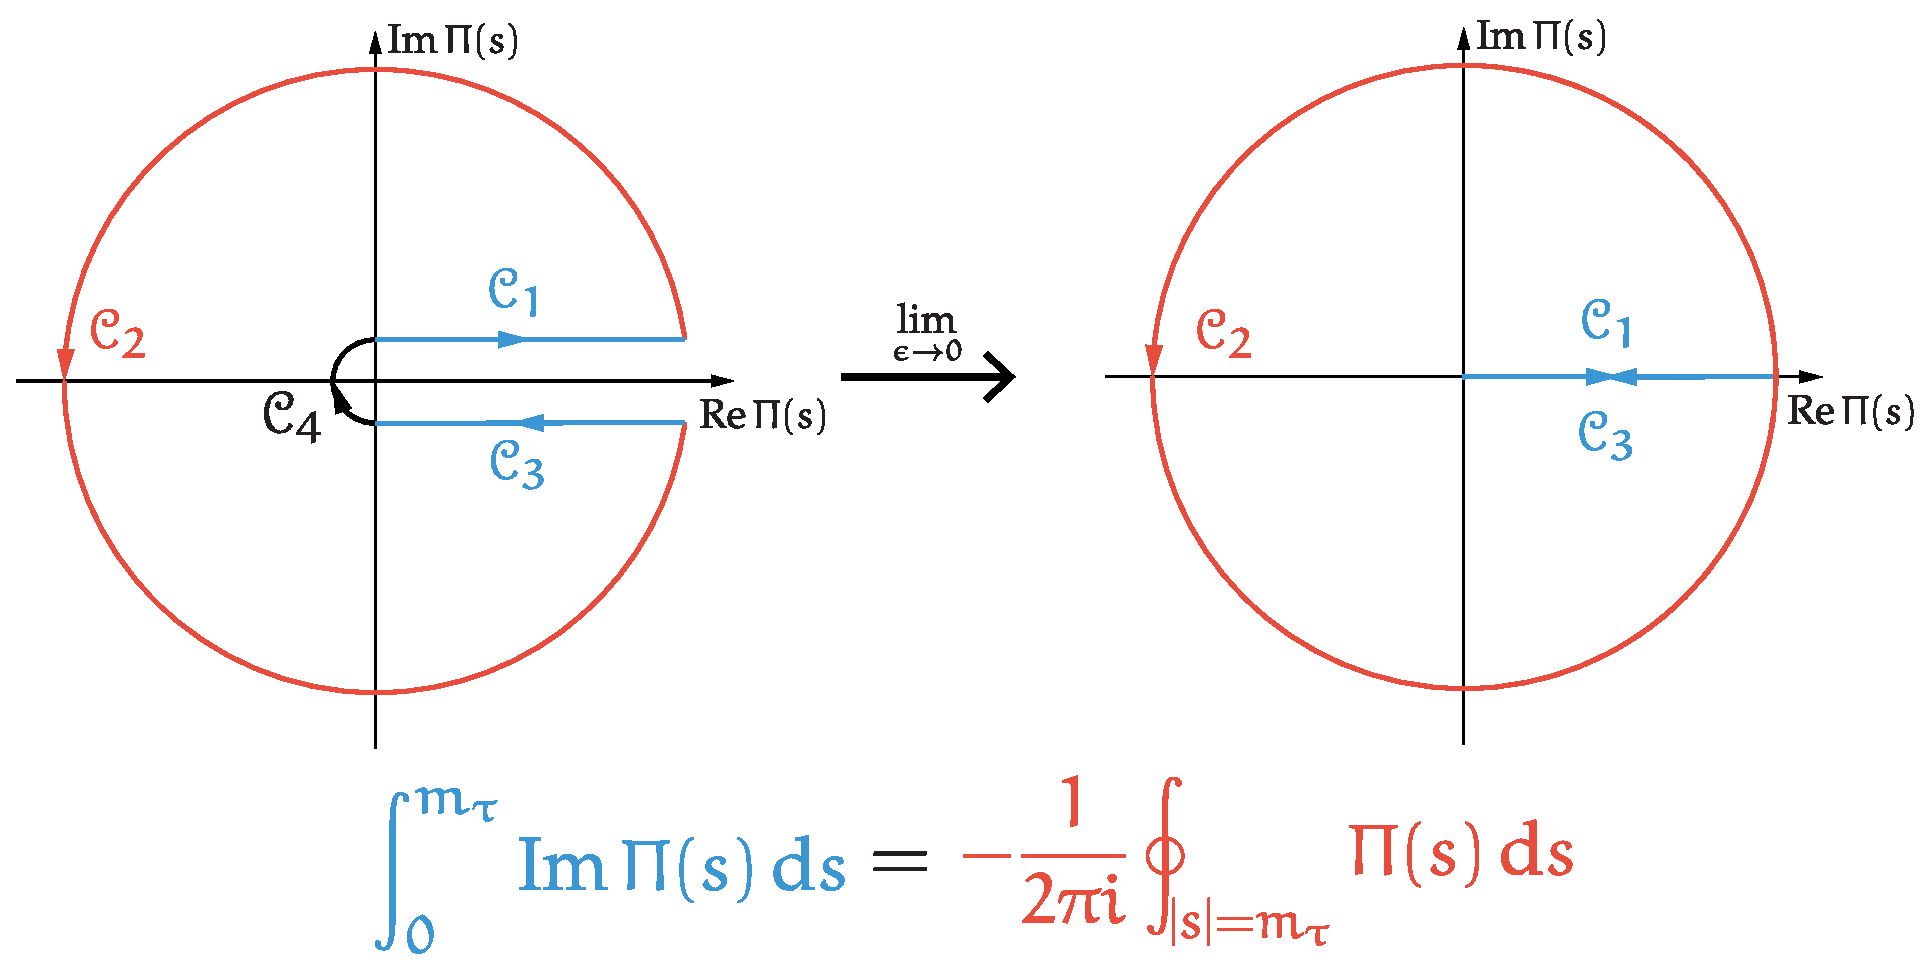
\includegraphics[width=0.8\textwidth]{./images/rTauCauchysTheorem.eps}
  \caption{Visualisation of the usage of Cauchy's theorem to transform
    \cref{eq:dispersionRelation} into a closed contour integral over a circle of
    radius $s_0$.}
  \label{fig:theoreticalTwoPointFunction}
\end{figure}
and mathematically we can express it as
\begin{equation}
  \label{eq:sumRulesCauchysTheorem}
  \oint \Pi(s) = \int_0^{s_0} \Pi(s+i\epsilon)-\Pi(s-i\epsilon)\dif s
  + \int_{0+\alpha(\epsilon)}^{2\pi-\alpha(\epsilon)}\Pi(s_0e^{i\theta})\dif \theta + \int_{3\pi/2}^{\pi/2}\Pi(s_0e^{i\theta})\dif \theta 
\end{equation}
If we make to use of \textit{Schwartz reflection principle}:
\begin{equation}
  f(\overline{z}) = \overline{f(z)},
\end{equation}
which can be applied if \(f\) is analytic and maps only to real values on the
positive real axis, we can express the integrand of the first integral of
\cref{eq:sumRulesCauchysTheorem} as the imaginary part of the two\-/point
function
\begin{equation}
  \Pi(s+i\epsilon)-\Pi(s-i\epsilon) = \Pi(s+i\epsilon)-\Pi^*(s+i\epsilon) = 2i\Ima\Pi(s+i\epsilon),
\end{equation}
which is by definition equal to the spectral function
\begin{equation}
  \rho(s) \equiv \frac{\Ima\Pi(s)}{\pi}.
\end{equation}
After taking the limit of small epsilon we can relate the line integral to a
finite momentum \(s0\) experimental spectral function to a theoretical
accessible circular contour integral of radius \(s_0\)
\begin{equation}
  \int_0^{s_0} \rho(s) = \frac{-1}{2\pi i}\oint_{\abs{s}=s_0} \Pi(s) \dif s, \quad \text{where we applied} \quad \epsilon \to 0.
\end{equation}
Note that the unphysical of the polynomial in \cref{eq:dispersionRelation}
cancel in the contour integral.

We are free to multiply the upper equation with an analytic function
\(\omega(s)\), which completes the \textsc{fesr}
\begin{tcolorbox}[ams equation,myformula]
  \label{eq:qcdSumRules}
  \int_0^{s_0} \omega(s) \rho(s) = \frac{-1}{2\pi i}\oint_{\abs{s}=s_0}\omega(s)
  \Pi_{OPE}(s) \dif s
\end{tcolorbox}
where the \define{lhs}{left\-/hand side} is given by the experiment and the
\textsc{rhs}. can be theoretically evaluated by applying the \textsc{ope} of the
correlator $\Pi_{OPE}(s)$. The analytic function \(\omega(s)\) plays the role of
a weight. It can be used to further suppress the non\-/perturbative
contributions coming from as \textit{duality violations} and also enhance or
suppress different contributions of the \textsc{ope} as we will see.

\subsection{Weighting OPE dimensions}
We can also use different weights to control the dimensions of the OPE that
contribute. The weights we are using have to be analytic, so that we can make
use of Cauchy's theorem. Thus they can be represented as polynomials
\begin{equation}
  \omega(x) = \sum_i a_i x^i,
\end{equation}
every contributing monomial is responsible for a dimension of the OPE.
Dimensions that are not represented in the weight polynomial do not contribute
at all or are very suppressed as we will demonstrate now.

The residue of a monomial \(x^k\) is only different from 0 if its power \(k=-1\):
\begin{equation}
  \label{eq:monomialWeights}
  \oint_{C} x^k \dif x = i \int_0^{2\pi}\left(e^{i \theta}\right)^{k+1} \dif \theta
  = \begin{cases} \mbox{$2 \pi i$} & \mbox{if } k=-1, \\ \mbox{0} & \mbox{otherwise} \end{cases}.
\end{equation}
Consequently if we exchange the kinematic weight of the include ratio
\cref{eq:inclusiveRatio} through a monomial and neglect all terms of no interest
to us we can write
\begin{equation}
  \label{eq:monomialInclusiveRatio}
  \begin{split}
    \left. R(x m_\tau) \right\rvert_{D=0,2,4\dots} &= \oint_{\abs{x}=1} \frac{x^k}{(x m_\tau)^{\frac{D}{2}}}C^{D}(x m_\tau) \\
    &= \frac{1}{(m_\tau)^{\frac{D}{2}}} \oint_{\abs{x}=1} x^{k-D/2} \,C^{D}(x
    m_\tau),
  \end{split}
\end{equation}
where $C^{D}$ are the $D$-dimensional Wilson coefficients. Thus combining
\cref{eq:monomialWeights} with \cref{eq:monomialInclusiveRatio} we see that only
Dimension which fulfill
\begin{equation}
  k - D/2 = -1 \quad \implies \quad  D = 2(k+1)
\end{equation}
contribute to the OPE. For example the polynomial of the kinematic weight is
given by
\begin{equation}
  (1 - x)^2 (1 + 2x) = \underbrace{1}_{D=2} - 3\underbrace{x^2}_{D=6} + 2\underbrace{x^3}_{D=8},
\end{equation}
where we underbraced the monomial and gave the active dimensions. A list of
monomomials and their corresponding Dimensions up to dimension 14 can be found
in \cref{table:monomialDimensions}.
\begin{table}
  \centering
  \begin{tabular}{l|ccccccc}
    \toprule
    \textbf{monomial:} & $x^0$ & $x^1$ & $x^2$ & $x^3$ & $x^5$ & $x^6$ & $x^7$\\
    \textbf{dimension:} & $D^{(2)}$ & $D^{(4)}$ & $D^{(6)}$ & $D^{(8)}$ & $D^{(10)}$ & $D^{(12)}$ & $D^{(14)}$\\
    \bottomrule 
  \end{tabular}
  \caption{List of monomial and their corresponding ``active'' dimensions in the
    OPE.}
  \label{table:monomialDimensions}
\end{table}
This behavior enables us to bring out different dimensions of the OPE and
suppress contributions of higher order ($D\geq10$) for which less is known.


For the interested reader we gathered several introduction texts to the
\textsc{qcdsr}, which where of great use to us
\cite{Narison1989,Rafael1997,Colangelo2000,Dominguez2013}.
\end{document}
% LocalWords:  qcdFeynmanDiagrams qcdFeynmanRules dispersionRelation sav itm
% LocalWords:  qcdCurrent twoPointFunction anomalousMassDimension sumRules lccc
% LocalWords:  OPEFeynmanDiagram correlatorComplexContour qcdSumRules ams iqx
% LocalWords:  LocalWords simpleTwoPointFunction twoPointFunctionSelfEnergy
% LocalWords:  cuttingRules qcdLagrangian electronElectronScattering myformula
% LocalWords:  lambdaRegularisation groundStateMesons strongCouplingFirstOrder
% LocalWords:  runningOfAs tauAntiTauAnnihilation analyticStructureCorrelator
% LocalWords:  kallenLehmannSpectralRepresentation rhoScalarCorrelator
% LocalWords:  kallenLehmanSpectralDecomposition theoreticalTwoPointFunction
% LocalWords:  sumRulesCauchysTheorem
